\section{Superposition as a Cause of Hallucinations}
\label{sec:superposition_as_a_cause_of_hallucinations}

After reviewing the paper, a key question emerged: could interference from superposition cause hallucinations in large language models?
To test this, we trained a classifier on high-sparsity data, inducing superposition, and evaluated it on low-sparsity data.

\subsection{Dataset}
As in the paper, we use a dataset with five distinct features and classes.
For this, we chose five English affixes: \textit{un-}, \textit{re-}, \textit{-able}, \textit{-ful}, \textit{-ness}, though any set of affixes would suffice.

We generated two datasets: one with words containing exactly one affix (pure words) and another with words containing multiple affixes (dual words, e.g., \textit{unreliable}).
The pure dataset was split into training and test sets, while the dual dataset was set aside for evaluation.

\subsection{Model}
We trained a model with an embedding layer, a convolutional layer, a hidden layer, and a ReLU activation function.
The hidden layer had only two neurons, forcing it to use superposition to encode all five features.

\subsection{Results}
After training the model on the pure dataset, we used the \href{https://colab.research.google.com/github/anthropics/toy-models-of-superposition/blob/main/toy_models.ipynb}{toy model framework} to visualize the representation of the five features in the hidden layer.
\begin{figure}[h]
	\centering
	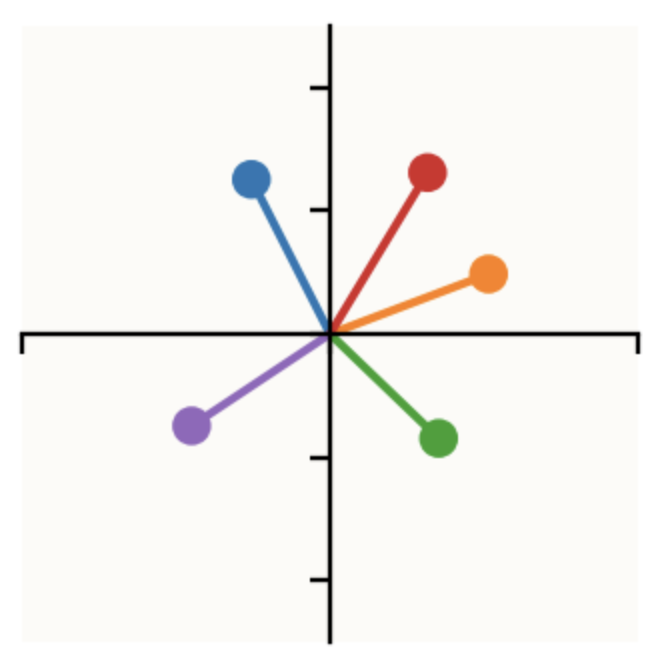
\includegraphics[width=0.5\linewidth]{figures/hidden_layer_representation.png}
	\caption{Representation of the five features in the hidden layer.}
	\label{fig:hidden_layer_representation}
\end{figure}
Figure \ref{fig:hidden_layer_representation} shows the model successfully encoded all five features, though it did not form the pentagon-like structure observed in the paper.
Table \ref{tab:hallucinations_results} shows the results of evaluating the model on the test set and the dual dataset.
\begin{table}[h]
	\centering
	\begin{tabular}{lc}
		\toprule
		\textbf{Dataset} & \textbf{Accuracy} \\
		\midrule
		Test set         & 0.9772            \\
		Dual dataset     & 0.9581            \\
		\bottomrule
	\end{tabular}
	\caption{Model evaluation on the test set and the dual dataset.}
	\label{tab:hallucinations_results}
\end{table}
The model performs well on the test set, but accuracy drops on the dual dataset, despite each dual word having twice the number of correct labels.
This suggests that when features are less sparse than during training, the additive interference from superposition can lead to misinterpretations of the input, which may contribute to hallucinations in large language models.
